\documentclass[runningheads,a4paper]{llncs}

\usepackage[utf8]{inputenc}
%\usepackage[T1]{fontenc}
\usepackage{amssymb}
%\setcounter{tocdepth}{3}
\usepackage{graphicx}   % for the adjustwidth environment

\usepackage{url}    
\urldef{\mailsa}\path|{anna.bernasconi,carlo.ghezzi}@polimi.it| 
\urldef{\mailsb}\path|pspoleti@kennesaw.edu| 
\urldef{\mailsd}\path|claudio.menghi@gu.se|
\urldef{\mailsc}\path|lenore@cs.uic.edu|   
\newcommand{\keywords}[1]{\par\addvspace\baselineskip
\noindent\keywordname\enspace\ignorespaces#1}

%%%%%%%%%%%%%%%%%%START CUSTOM SECTION%%%%%%%%%%%%%%%

\usepackage{mathtools}
\usepackage{mathpartir}
\usepackage[inline]{enumitem}
\usepackage{cancel}
\usepackage{algorithm}
\usepackage{algpseudocode}
\usepackage{todonotes}

 \usepackage{ltl}
\usepackage{multicol}
\usepackage{amsmath}
\usepackage{textgreek}
\usepackage{enumitem}
\usepackage{pifont}
\usepackage{changebar}
\usepackage{changes}
\usepackage{multirow}
\usepackage{makecell}

\definecolor{mygreen}{rgb}{0.0, 0.5, 0.0}
\definecolor{myred}{rgb}{0.8, 0.0, 0.0}

\usepackage{scalerel}
\def\thumbsup{\scalerel*{
\includegraphics{up.png}}{O}}
\def\thumbsdown{\scalerel*{
\includegraphics{down.png}}{g}}

\newcommand{\validProof}{\ding{51}}
\newcommand{\validCounterexample}{\textcolor{mygreen}{\thumbsup}}
\newcommand{\notvalidProof}{\ding{55}}%
\newcommand{\spuriosCounterexample}{\textcolor{myred}{\thumbsdown}}%
\newcommand{\gba}{\ensuremath{\mathcal{E}_{\lnot\phi}}}
\newcommand{\ba}{\ensuremath{\mathcal{\mathcal{A}_{\lnot\phi}}}}
\usepackage{todonotes}
\author{Claudio Menghi}
\definechangesauthor[name={Claudio Menghi},color=orange]{CM}
\author{Anna Bernasconi}
\definechangesauthor[name={Anna Bernasconi},color=red]{AB}
\author{Paola Spoletini}
\definechangesauthor[name={Paola Spoletini},color=green]{PS}

\newcommand\numberthis{\addtocounter{equation}{1}\tag{\theequation}}

\usepackage{tikz, pgf, pgfplots}
\usetikzlibrary{automata,positioning}
\usetikzlibrary{shapes,shapes.geometric}
\usetikzlibrary{backgrounds}

%%circled numbers in line with text
\newcommand*\circled[1]{\tikz[baseline=(char.base)]{
            \node[shape=circle,draw,inner sep=1pt] (char) {#1};}}
            
%utils for automata states
\tikzset{state/.style={
        draw, 
        ellipse, 
        minimum height=2em, 
        minimum width=2.8em,  
        thick } }
\tikzset{statep/.style={
    draw, 
    ellipse, 
    minimum height=1em, 
    minimum width=1em,  
    thick } }
\tikzset{emptynode/.style={ draw } }
\tikzset{empty/.style={ } } 

% per testo barrato
\usepackage[normalem]{ulem}
\newcommand{\cla}[1]{{\color{blue} #1}}
\newcommand{\anna}[1]{{\color{red} #1}}
\newcommand{\pao}[1]{{\color{green} #1}}
\newcommand{\fixme}[1]{{\color{red} #1}}


\newcommand{\NAME}{THRIVE}

\newcolumntype{P}[1]{>{\centering\arraybackslash}p{#1}}

%%%%%%%%%%%%%%%%%%END CUSTOM SECTION%%%%%%%%%%%%%%%


\begin{document}

\mainmatter  % start of an individual contribution

% first the title is needed
\title{From model checking to a temporal proof \\for partial models}

% a short form should be given in case it is too long for the running head
\titlerunning{From model checking to a temporal proof for partial models}

% the name(s) of the author(s) follow(s) next
%
% NB: Chinese authors should write their first names(s) in front of
% their surnames. This ensures that the names appear correctly in
% the running heads and the author index.
%




\author{Anna Bernasconi\inst{1}
\and Claudio Menghi\inst{2}
\and Paola Spoletini\inst{3}
\and \\ Lenore D. Zuck\inst{4}
\and Carlo Ghezzi\inst{1}}
%
\authorrunning{From model checking to a temporal proof for partial models}
% (feature abused for this document to repeat the title also on left hand pages)

% the affiliations are given next; don't give your e-mail address
% unless you accept that it will be published
\institute{Politecnico di Milano, DEIB - DEEPSE group,\\
\mailsa\\
\and
Chalmers University of Technology | University of Gothenburg\\
\mailsd\\
\and
Kennesaw State University,\\
\mailsb\\
\and
University of Illinois at Chicago,\\
\mailsc\\
}


\toctitle{Lecture Notes in Computer Science}
\tocauthor{Authors' Instructions}
\maketitle


\begin{abstract}
Three-valued model checking has been proposed to support verification when some portions of the model are unspecified. 
Given a formal property, the model checker returns \emph{true} if the property is satisfied, \emph{false} and a violating behavior if it is not,  \emph{maybe}  and a possibly violating behavior if
it is \emph{possibly satisfied}, i.e., its satisfaction may depend on how the unspecified parts are refined.
Model checking, however, does not explain the reasons \emph{why} a property holds, or possibly holds.
Theorem proving can instead do it by providing a formal proof that explains why a property holds, or possibly holds in a system. Integration of theorem proving with model checking has only been studied for classical two-valued logic -- hence, for fully specified models.
%Theorem proving has been used in two-valued model checking to produce a formal proof in the case the property holds in a system. 
This paper proposes a unified approach that enriches three-valued model checking with  theorem proving to generate proofs which explain why \emph{true} and \emph{maybe} results are returned.
\end{abstract}

\section{Introduction}
\label{sec:intro}
Multi-valued model checking techniques, such as~\cite{bruns1999model,bruns2000model,gurfinkel2003multi,bruns2004MCmultivalued,DBLP:conf/fm/MenghiSG16}, have been proposed to support the verification of models that are \emph{partial}, i.e.,  their state space is not fully specified.
Three-valued model checking is a multi-valued model checking technique that extends classical two-valued model checking by possibly returning an additional \emph{maybe} value.
More precisely, it returns  \emph{true} if the property definitely holds, \emph{false} if it definitely does not hold,  \emph{maybe} otherwise.




In the classical context of two-valued model checking, although a sample violating behavior (a counterexample) is normally returned when the property is violated, no equally useful insight is provided if the property holds. 
In practice, it would be useful to receive a formal explanation of the reason \emph{why} the system satisfies the property.
To achieve this goal, the model checking framework can be equipped with a theorem prover that formally justifies why model checking has failed in the search of a counterexample.
Theorem proving algorithms have been developed for fully specified models~\cite{peled2001falsification,peled2001model}, but no known similar approach deals with partial models.

The ability to deal with partial models has a strong practical motivation. Software development often proceeds in an iterative and incremental fashion. Designers may start by providing an initial, high-level version of the model, which is iteratively narrowed down as design progresses and uncertainties are removed.
Whenever the result of verification  is \emph{true} or \emph{maybe}, the proof can guide the designer throughout the refinement process, and confirm the correctness of the design choices already performed. 
In some cases, the proof may even implicitly suggest that actually the property does not capture the intended correctness condition, and it should be modified.
For this reason, the integration of theorem proving techniques and multi-valued model checking can guide the designer towards the development of a correct model.

This paper proposes \NAME , a THRee valued Integrated Verification framEwork for partial models.
\NAME\ enriches model checking for partial models with theorem proving.
Theorem proving is used when a \emph{true} or a \emph{maybe} value is returned by the model checker to justify why the verified system \emph{definitely}  or \emph{possibly} satisfies the property of interest.
%Whenever the property \emph{definitely holds}, the deductive verification approach proves that neither a definitely violating nor a possibly violating behavior can be found in the current instance of the model.
%If the property \emph{possibly holds}, the model checker returns a possible counterexample, which describes a possible behavior that violates the property. 
%In addition, the deductive verification engine returns to the designer a proof that specifies why a violating behavior cannot be found in the current model.
%Finally, whenever the property \emph{does not hold}, a counterexample is returned, which specifies a violating behavior.
In addition to the general framework, we present  a specific instance of \NAME\ useful for applications, which considers models described as Partial Kripke Structures (PKSs)~\cite{bruns1999model} and properties expressed as Linear Temporal Logic (LTL)~\cite{pnueli1977temporal} formulae.
The instance is based on the three-valued LTL semantics~\cite{bruns1999model}.
To successfully integrate model checking and theorem proving we customize the theorem proving framework (based on deductive verification) proposed in~\cite{peled2001model} to support PKSs and LTL formulae.

We consider the applicability of \NAME\  w.r.t.  \emph{three-valued}~\cite{bruns1999model} and  \emph{thorough}~\cite{bruns2000model} LTL semantics. 
We also discuss its applicability in the case of \emph{self-minimizing}~\cite{godefroid2005MCvsGMC} LTL formulae, which are known to represent a practically relevant subset of LTL formulae~\cite{antonik2006efficient}. 
We evaluate the benefits of the framework on an example by simulating  the design of a medical software critical component~\cite{arcaini2015formal}.
A discussion on the use of \NAME\ in real world scenarios concludes the evaluation.




\begin{figure}[t]
 \centering
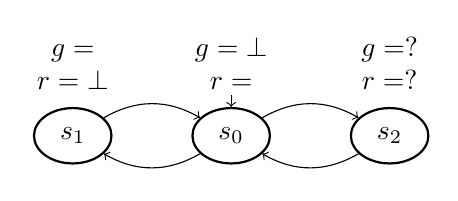
\begin{tikzpicture}[scale=0.33] %[x={10.0pt},y={10.0pt}]

\node [state, initial, initial text={},initial where=above](s_0)
[label={
[align=center,yshift=0.1cm]
%above:
% \includegraphics[width=50pt]{images/Red.pdf}
%$\boldsymbol{\overline{green}=T}$\\
$g=\color{black}\bot$\\
$r=\LTLtrue$
}] 
{$s_0$};   


\node[state] (s_1) 
[left=of s_0,
label={
[align=center,yshift=0.1cm]
%above:
% \includegraphics[width=50pt]{images/Green.pdf}
%$\boldsymbol{\overline{green}=F}$\\
$g=\color{black}\LTLtrue$\\
$r=\bot$
}]  
{$s_1$};

\node[state] (s_2) 
[right=of s_0,
label={
[align=center,yshift=0.1cm]
%above:
% \includegraphics[width=50pt]{images/Bo.pdf}
%$\boldsymbol{\overline{green}=\bot}$\\
$g=\color{black}?$\\
$r=?$
}]  
{$s_2$};


\path[->]      
(s_0) edge [bend left] node [above]{} (s_1) 
(s_1) edge [bend left] node [above]{} (s_0)
(s_0) edge [bend left] node [above]{} (s_2)
(s_2) edge [bend left] node [above]{} (s_0);   

\end{tikzpicture}
\caption{System model $M$}
\label{fig:modelmot}
\end{figure}


\textbf{Running example}. \emph{We consider a  simple grade crossing semaphore.
We assume that the designer has identified three simple properties:
\begin{enumerate*}[label={(\arabic*)}]
\item $Red$ lights up infinitely often -- formalized as $\phi_1=\LTLglobally\LTLfinally red$.
\item $Green$ lights up infinitely often -- formalized as $\phi_2=\LTLglobally\LTLfinally green$.
\item When the light is $red$, it will always be $green$ -- formalized as $\phi_3=\LTLglobally (red \LTLimplication \LTLglobally green)$.
\end{enumerate*}
Note that $\phi_3$ is deliberately wrong %(i.e., it does not capture the desired behavior).
and will be used later to discuss the application of \NAME .\hfill
\break
Starting from this specification, a designer might initially propose the partially specified model of the semaphore shown in Figure~\ref{fig:modelmot}. Each state is associated with the values of the propositions $g$ and $r$ (denoting $green$ and $red$) holding in that state, which specify whether the green and the red lights are on or off.
For example, in state $s_0$ the red light is on ($r=\LTLtrue$) while the green is off ($g=\LTLfalse$).
Instead,  $s_2$ is a state to which the semaphore may be brought, for instance by a manual command. 
The designer still has to choose whether, in this state, the green and red lights should be on or off.
This is indicated by associating the value $?$ to the propositions $g$ and $r$.
The designer might refine the model by setting $g$ and $r$ to either $\LTLtrue$ or $\LTLfalse$ in $s_2$.}

\textbf{Related work.}
Three-valued~\cite{larsen1988modal,godefroid2001abstraction,bruns1999model,bruns2000model,godefroid2011ltl} and multi-valued~\cite{gurfinkel2003multi,bruns2004MCmultivalued} model checking supports verification of partial models. 
Different model checking techniques have been developed depending on the modeling formalisms.
For example, several papers  focus on Partial Kripke Structures (e.g.,~\cite{bruns1999model,bruns2000model,godefroid2011ltl,gurfinkel2003multi,bruns2004MCmultivalued}), others on Modal Transition Systems (e.g.,~\cite{larsen1988modal,godefroid2001abstraction}). 
However, to the best of our knowledge, none of these techniques has been combined with theorem proving.  

Theorem proving applies a set of techniques to try to establish the validity of a given formula (see~\cite{manna2012temporal}).
Some of these techniques (e.g., ~\cite{peled2001falsification,peled2001model,namjoshi2001certifying,cleaveland2002evidence,rajan1995integration}) exploit the state space generated by the model checker to explain why a property holds.
However, to the best of our knowledge, none of these approaches has been applied in a multi-valued context.


\textbf{Organization.}
Section~\ref{sec:preliminaries} contains background notations and algorithms.
%presents the background. notations and algorithms.
Section~\ref{sec:contribution} describes \NAME.
Section~\ref{sec:theoremProverAdapting} presents an instance of \NAME , that considers PKSs and LTL formulae. 
Section~\ref{sec:preliminaryEvaluation} evaluates the approach on an example.
Section~\ref{sec:discussion} discusses the applicability of \NAME\ in real world cases.
%Finally, Section~\ref{sec:conclusions} concludes the paper.
Section~\ref{sec:conclusions} concludes the paper.

%\section{Motivating Example.} 
%\label{sec:motivating}
%
%While the behavior in $s_0$ and $s_1$ is fully specified, the designer is uncertain on how the semaphore works in $s_2$.
%More precisely, in the state $s_0$ the semaphore is red while in $s_1$ it is green. 
%The semaphore repeatedly moves from $s_0$ to $s_1$ and vice versa. 
%However, at some point, the semaphore may be manually moved into the state $s_2$.
%This may occur when an anomalous event is detected, such as an accident or an emergency condition.
%At the current development stage state $s_2$ is unspecified.
%Should the $red$, the $green$ light, or both of them be turned on?
%Note that the design of the system behavior in state $s_2$ may also be assigned to a third party company.


%Liveness and safety requirements are among the most interesting and common temporal properties that we might request. 
%For illustration purposes, we would like to make sure that in $M$ $red$ infinitely often lights up ($\phi_1$). On the other hand, we also want to enforce that contradictory messages are not sent out forever: \emph{does it ever happen that eventually permanently red and green are lightened up simultaneously?} ($\phi_2$).
%In addition, we also request a simple liveness property $\phi_3$, ``infinitely often green'', since it is important that the passage is always eventually allowed.

%We are proposing a comprehensive framework that allows the designer to examine these properties satisfiability in $M$. 



Regardless of the temporary incompleteness, the designer wants to evaluate the satisfaction of the properties of  interest. 
By model checking, it is possible to verify that the model does not contain any behavior that violates or possibly violates $\phi_1$. 
However, the result does not provide any information on why $\phi_1$ is satisfied.
Instead, a model checker equipped with a deductive verification framework would reveal that the system enters infinitely often state $s_0$, in which the red light is turned on, thus explaining why property $\phi_1$ is satisfied.

Let us now consider property $\phi_2$, which possibly holds.
The model checking algorithm returns a \emph{possible} counterexample: by turning off the green light in state $s_2$, the system may infinitely loop over $s_0$ and $s_2$ without $g$ ever being true. 
However, the search of a \emph{definitive} counterexample has failed.
The deductive verification framework would explain to the designer why this search failed.
As a matter of fact, if a counterexample is present, it must be present in any possible completion  of the model, i.e., for any possible assignment to the light in the state $s_2$.
But, let us consider a possible refinement of the incomplete state $s_2$ where the green light is on.
Since the green light is on in $s_1$ ($s_2$), it is possible to deduce that the light is eventually green in state $s_1$ ($s_2$).
Since it is allowed to loop over states $s_0$, $s_1$ and $s_2$, it is possible to deduce that ``always eventually green" is true in $s_0$, $s_1$ and $s_2$.
Thus, $\phi_2$ is satisfied in $s_0$, the initial state.
In conclusion, when the model checker returns maybe, it outputs a possible counterexample for a possible refinement of the incomplete states. 
In addition, the deductive verification framework would explain that the search of a definitive counterexample has failed in the case in which the green light is on in $s_2$.
This provides a useful insight to the designer, explaining that, by setting $g$ to $\LTLtrue$ in $s_2$, one obtains a model satisfying $\phi_2$ while, in the opposite case, $\phi_2$ is violated.


Finally, when property $\phi_3$ is considered, the model checking algorithm returns a definitive counterexample since $\phi_3$ is not satisfied, regardless of further refinements of $s_2$. Indeed, there exists an infinite run among states $s_0$ and $s_1$ in which a red light is not followed by a permanently green light. Indeed, the requirement that the designer probably meant to specify is $\LTLglobally (red \LTLimplication \LTLnext green)$.



%
%The model checker returns an ``unknown'' answer because if, in a future implementation, the semaphore is green in $s_2$, then the property holds. On the contrary, should not the green light be configured in $s_2$, the property would be violated.
%
%What our proposed approach offers is the ability to jointly analyze both potentially bad designs and potentially good designs.
%Especially in those cases where the model checker answer is ``unknown'', the designer is provided with information that can reveal itself fundamental to complete the current design. Namely: he/she obtains a counterexample that shows one violating behavior along with a proof that justifies why the current implementation of the model does not violate the property.
%The counterexample returned corresponds to the scenario in which the system infinitely loops over states $s_0$ and $s_2$.
%The provided proof explains  to the designer \emph{why} the search of a violating behavior has failed.
%This procedure considers a version of $M$ in which the $?$ values are substituted with $\LTLtrue$.
%It first identifies a set of axioms that specify why the search fails in some states of the model.
%By using a set of deductive verification rules it shows how these axioms imply the overall satisfaction of $\phi_3$.
%In this example, we first state what axiomatically holds in the states $s_1$ and $s_2$, which are the peripheral areas of the model.
%Since $s_1$ and $s_2$ are successors of $s_0$ we can inductively deduce what is satisfied in $s_0$. The final result, is reached by conjucting all the conclusiones gathered on the single model states.
%

%%%%


\section{Background}
\label{sec:preliminaries}

\vskip 0.05in  
\textbf{\indent Checking complete models.}
 Given a Kripke Structure $M$ (KS), the model checking procedure verifies whether a Linear Temporal Logic (LTL) formula $\phi$ holds or does not hold in $M$. 
The procedure works in three steps:
\begin{enumerate*}[label={(\arabic*)}]
\item generation of a B{\"u}chi automaton (BA) $\mathcal{A}_{\lnot\phi}$ from the LTL formula $\neg \phi$;
\item generation of the product $\mathcal{G}=M \otimes\mathcal{A}_{\lnot\phi}$;
\item emptiness check of $\mathcal{G}$.
\end{enumerate*}




\vskip 0.05in  
\textbf{Checking partial models.}
\emph{Partial Kripke Structures}~\cite{bruns1999model}  (PKSs) extend KSs by allowing a proposition in a given state to be labelled with $?$ to represent an unknown value. 
A PKS $M$ is a tuple $\langle S, R,S_0,AP,L \rangle$,
where:
\begin{enumerate*}
\item[] $S$ is a set of \emph{states};
\item[] $R\subseteq S\times S$ is a \emph{left-total} \emph{transition relation} on $S$;
\item[] $S_0$ is a set of initial states;
\item[] $AP$ is a set of atomic propositions;
\item[] $L: S\times AP\rightarrow \{\top,?,\bot\}$ is a \emph{function} that, for each state in $S$, associates a truth value in the set $\{\top,?,\bot\}$ to every atomic proposition in $AP$.
\end{enumerate*}  
The model of the grade crossing semaphore presented in Figure~\ref{fig:modelmot}  is an example of a PKS.

A \emph{completion} of a PKS $M$ is a KS $M^\prime$ that completes $M$ by assigning values to the unknown propositions.
The set $\mathcal{C}(M)$ contains all the completions of $M$.

Two kinds of LTL semantics (three valued and thorough) exist for  PKSs. 
%When the satisfaction of LTL formulae is considered w.r.t. PKSs, either the three-valued or the thorough semantics can be considered.
%----------------------------------------------------------------------------------------------------------------------------------------------------------------
% Three-valued LTL semantic
%----------------------------------------------------------------------------------------------------------------------------------------------------------------


\emph{Three-valued LTL semantics} $[(M,\pi) \models \phi]$ associates to a model $M$, a path $\pi$ of  $M$, and a formula $\phi$, a truth value in the set $\{ \bot, ?, \top \}$. This semantics specifies that a formula $\phi$ definitely holds in a PKS $M$ if it is true for all possible values of the unknown propositions in $M$. 
Likewise, it is definitely violated if it is false despite the unknown values.
%A formula $\phi$ is not satisfied if there is a path $\pi$ in the PKS which violates $\phi$ despite the unknown values of the atomic propositions associated to the states of $\pi$.
%Otherwise the formula is unknown.
According to three-valued semantics~\cite{godefroid2011ltl}, given a PKS $M = \langle S, R,$ $S_0, AP, L \rangle$, a path $\pi=s_0,s_1,\ldots$, and a formula $\phi$, we inductively define that $\pi$ satisfies $\phi$ in the model $M$ as follows:
\begin{align*}
&[(M,\pi) \models p] &   = &&& L(s_0,p)\\
&[(M,\pi) \models \lnot\phi] &   = &&& \textnormal{comp}([(M,\pi) \models\phi]) \\
&[(M,\pi) \models \phi_1 \LTLand \phi_2] &   =   &&& \min([(M,\pi) \models\phi_1],[(M,\pi) \models\phi_2])\\
&[(M,\pi) \models \LTLnext \phi] &   =  &&& [(M,\pi^1) \models\phi]\\
&[(M,\pi) \models \phi_1 \LTLuntil \phi_2] &   =  &&& \max_{j\geq 0}(\min(\{[(M,\pi^i) \models\phi_1]|i<j\} \cup \{[(M,\pi^j) \models\phi_2]\}))
\end{align*}
\noindent{where the notation $\pi^i$ indicates the sub-path $s_i, s_{i+1} \ldots $ of $\pi$.}

Negation is defined by the function comp (complement), which maps $\top$ to $\bot$, $\bot$ to $\top$, and $?$ to $?$.
The conjunction (disjunction) is defined as the minimum (maximum) of its arguments, following the order $\bot <\ ? < \top$. These functions are extended to sets considering min($\emptyset$)=$\top$ and max($\emptyset$)=$\bot$.

Given a PKS $M = \langle S, R,$ $S_0, AP, L \rangle$, satisfaction of formula $\phi$ in a state $s$ is defined as  $[(M, s) \models \phi]  =   \min(\{[(M, \pi) \models \phi] \mid \pi^0=s\})$.
A PKS $M$ \emph{definitely satisfies} a property $\phi$ ($[M \models \phi]=\top$) iff for all initial states $s_0 \in S_0$ of $M$, $[(M, s_0) \models \phi]=\top$. 
A PKS $M$ \emph{does not satisfy} the property $\phi$ ($[M \models \phi]=\bot$) iff there exists an initial state $s_0 \in S_0$ of $M$ such that  $[(M, s_0) \models \phi]=\bot$.
A PKS \emph{possibly satisfies} $\phi$ otherwise.
%In the rest of the paper we will use interchangeably the expressions ``$M$ definitely satisfies $\phi$'' and ``$\phi$ holds in $M$'', ``$M$ does not satisfy $\phi$'' and ``$\phi$ does not hold in $M$'', as well as ``$M$ possibly satisfies $\phi$'' and ``$\phi$ possibly holds in $M$''.



Three-valued semantics does not behave always in accordance with the natural intuition~\cite{bruns2000model}: there are cases in which $\phi$ possibly holds for a PKS but all its  completions 
%(obtained by replacing the $?$ values with $\top$ and $\bot$) 
actually satisfy (or do not satisfy)  $\phi$.
%For instance, this happens when $\phi$ is a tautology or it is unsatisfiable with a traditional two-valued interpretation. 
For this reason, an alternative semantics, called \emph{thorough LTL semantics}~\cite{bruns2000model} has been proposed. 
According to it, a formula is possibly satisfied only if there exist two completions $M_1, M_2 \in \mathcal{C}(M)$, such that $\phi$ is definitely satisfied in one and violated in the other.
%Thorough semantics defines satisfaction of an  LTL formula $\phi$ by a PKS $M$ ($[M\models\phi]_t$)  as follows:
Thorough semantics defines satisfaction of an  LTL formula $\phi$ by a PKS $M$ as follows:
\begin{equation}
 [M \models\phi]_t  = 
                						\begin{cases}
                  								\top & \quad  \text{if}\ M^\prime \models \phi \text{ for all } M^\prime \in \mathcal{C}(M)\\
                  								\bot & \quad  \text{if}\ M^\prime \not\models\phi \text{ for all } M^\prime \in \mathcal{C}(M)\\
                  								? &  \quad  \text{otherwise}
                							  \end{cases}      					  		   \nonumber
\end{equation}


Given a PKS and an LTL formula $\phi$, it has been proved~\cite{godefroid2011ltl} that 
\begin{enumerate*}[label={(\arabic*)}]
\item $[M\models\phi] =$ $ \top \Rightarrow$ $ [M\models\phi]_t = \top$;
\item $[M\models\phi] = \bot \Rightarrow [M\models\phi]_t = \bot$.
\end{enumerate*}
That is, a formula which is true (false) under the three-valued semantics is also true (false) under the thorough semantics.

There exists a subset of LTL formulae, known in the literature as \emph{self-minimizing}~\cite{godefroid2005MCvsGMC}, such that the two semantics coincide. Formally,
given a model $M$ and a  self-minimizing LTL property $\phi$, then $[M\models\phi]=[M\models\phi]_t$. It has been observed that most practically useful LTL formulae belong to this subset~\cite{godefroid2005MCvsGMC}.

%In~\cite{godefroid2005MCvsGMC} the authors showed that many temporal-logic formulae of practical interest are self-minimizing.
%More precisely, all the formulae that do not contain atomic propositions with mixed polarity (negated and not negated) in their negation normal form are self-%minimizing; if the formulae follow specific patterns are self-minimizing;
%some LTL formulae that are not self-minimizing can be converted into self-minimizing LTL formulae using a procedure called semantic-minimization.
%The interested reader may refer to~\cite{godefroid2005MCvsGMC} for more details.
%
%


We present a \emph{model checking} algorithm for PKSs and LTL formulae based on three-valued semantics. 
%This algorithm exploits two classical model checking procedures for KSs.
This procedure considers a version of $M$, called \emph{complement-closed}~\cite{bruns2000model}, in which for every proposition $p \in AP$, there exists a new proposition $\overline{p}$, called complement-closed proposition, such that $L(s,\overline{p})=$ comp$(L(s,p))$, for all $s \in S$.
%	The proposition $q$, whose value is complementary to the one of $p$, is indicated as $\overline{p}$.
For example, the complement-closed version of the PKS of the semaphore example is presented in Figure~\ref{fig:model}.
%, where the atomic propositions $\overline{g}$ and $\overline{r}$ are associated with the complement of the values of  propositions green ($g$) and red ($r$), respectively.

\begin{figure}[t]
\begin{minipage}[b]{.5\textwidth}
  \begin{figure}[H]
 \centering
\begin{tikzpicture}[scale=0.33] %[x={10.0pt},y={10.0pt}]

\node [state, initial, initial text={},initial where=above](s_0)
[label={
[align=left,yshift=0.1cm]
above:
$\boldsymbol{\overline{g}=\top}$\\
$\boldsymbol{\overline{r}=\bot}$\\
$g=\color{black}\bot$\\
$r=\top$}] 
{$s_0$};   

\node[state] (s_1) 
[left=of s_0,
label={
[align=left,yshift=0.1cm]
above:
$\boldsymbol{\overline{g}=\bot}$\\
$\boldsymbol{\overline{r}=\top}$\\
$g=\color{black}\top$\\
$r=\bot$}]  
{$s_1$};

\node[state] (s_2) 
[right=of s_0,
label={
[align=left,yshift=0.1cm]
above:
$\boldsymbol{\overline{g}=?}$\\
$\boldsymbol{\overline{r}=?}$\\
$g=\color{black}?$\\
$r=?$}]  
{$s_2$};


\path[->]      
(s_0) edge [bend left] node [above]{} (s_1) 
(s_1) edge [bend left] node [above]{} (s_0)
(s_0) edge [bend left] node [above]{} (s_2)
(s_2) edge [bend left] node [above]{} (s_0)   

\end{tikzpicture}



\caption{The PKS of  the  crossing semaphore.}
\label{fig:model}
\end{figure}
\end{minipage}
\begin{minipage}[b]{.5\textwidth}
  \begin{figure}[H]
\centering
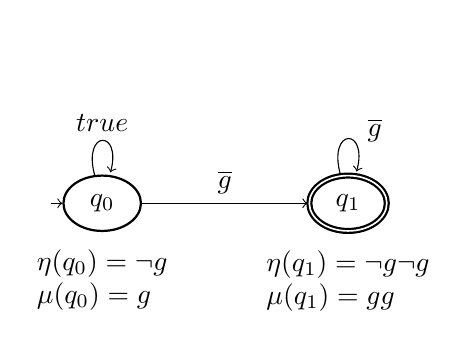
\begin{tikzpicture}[scale=0.33] %[x={10.0pt},y={10.0pt}]

\node[state, initial, initial text={}] (q_0) 
[label={
[align=left,yshift=-0.1cm]
below:
$\eta(q_0)= \LTLnext \LTLfinally \LTLglobally \lnot g$\\
$\mu(q_0)= \LTLnext \LTLglobally \LTLfinally g$}]
{$q_0$};
   
\node[state,accepting] (q_1) 
[right = 2.1cm of q_0,
label={
[align=left,yshift=-0.1cm]
below:
$\eta(q_1)= \lnot g \LTLand \LTLnext \LTLglobally \lnot g  $\\
$\mu(q_1)= g \LTLor \LTLnext \LTLfinally g$}]
{$q_1$};

\path[->]      
(q_0) edge [loop above]node [above]{$true$} (q_0) 
(q_0) edge node [above,align=center]
{\\ \\ \\ $\overline{g}$} (q_1)
(q_1) edge [loop above]node [above right, pos=0.8,align=center]
{\\ \\ \\ $\overline{g}$} (q_1);    

\end{tikzpicture} 
\caption{The BA associated with $\phi_2$.}
\label{fig:property}
\end{figure}
\end{minipage}
\end{figure}



%
%\begin{definition}[PKS optimistic and pessimistic labelling~\cite{bruns2000model}]
%Given a three-valued labelling function $L$,  we define the derived optimistic ($L_{opt}$) and pessimistic ($L_{pes}$) labelling function for every state s of the model $M$ as follows: 
%\begin{equation}
%    L_{opt}(s,p) \buildrel \text{def}\over = 
%                					\begin{cases}
%                  						\top & \quad  \text{if}\ L(s,p)=?\\
%                  						L(s,p) &  \quad otherwise
%                					\end{cases}
%\end{equation}            					  
%\begin{equation}      					  
%   L_{pes}(s,p) \buildrel \text{def}\over = 
%	                            \begin{cases}
%                  				       \bot  & \quad \text{if}\ L(s,p)=?\\
%                  						L(s,p) & \quad otherwise
%                					\end{cases}
%\end{equation}
%\end{definition}


The model checking procedure for a PKS $M$ is based on an optimistic and pessimistic approximation of $M$'s complement-closure.
The optimistic (pessimistic) approximation function $L_{opt}$  ($L_{pes}$) associates the value $\top$ ($\bot$) to each atomic proposition of the complement-closure of $M$ with value $?$.
Given a PKS $M=\langle S,R, S_0, L \rangle$, we have $M_{pes}=\langle S,R, S_0, L_{pes} \rangle$ for the pessimistic case, and $M_{opt}=\langle S,R, S_0, L_{opt} \rangle$ for the optimistic one.
%
%The model checking procedure exploits the under and the over approximations as we show hereafter.

The three-valued model checking algorithm assumes that property $\phi$ is rewritten using complement-closed propositions. 
The procedure works in two steps.
First, the formula is expressed such that negations only appear in front of atomic propositions. 
Second, each negated proposition is substituted by the corresponding complemented proposition.
Let $\phi$ be an LTL formula obtained using the procedure just discussed, $M=\langle S, R, S_0, L\rangle $ a PKS with $s \in S$, and $M_{pes}$ and $M_{opt}$ the corresponding pessimistic and optimistic cases. 
%
%Then, $[(M,s)\models\phi]$ has been defined in~\cite{bruns2000model}
\setcounter{footnote}{0}
Then, \cite{bruns2000model}\footnote{In~\cite{bruns2000model} the procedure is presented for PML but is valid also for LTL (see \cite{bruns2000model,godefroid2005MCvsGMC,godefroid2011ltl}).} has defined:
\begin{equation}
    [(M,s)\models\phi]  = 
                						 \begin{cases}
                  				 				\top & \quad \text{if}\ (M_{pes},s)\models\phi\\
                  								\bot & \quad \text{if}\ (M_{opt},s)\not\models\phi\\
                  								? & \quad  otherwise
                						\end{cases} \nonumber
\end{equation}

This technique exploits two runs of the classical two-valued model checking performed  on a pessimistic and an optimistic completion of  $M$.
%Note that whenever a $\top$ or $\bot$ value is returned, the property $\phi$ is guaranteed to be true/false in all the completions of $M$.
%For additional details on this procedure see~\cite{bruns2000model,godefroid2011ltl}.




%\begin{theorem}(The verification procedure is correct)
%\end{theorem}
%\begin{proof}
%Given a self-minimizing temporal logic formula $\phi$, by Proposition~\ref{def:self-minimizing}, generalized (which is based on the thorough semantic) and
%three-valued model checking produce the same result.
%Thus, the considered three-valued model checking algorithm returns the correct value also under the thorough interpretation.
%\end{proof}





\vskip 0.05in  
\textbf{Deductive verification.}
%Hereafter we briefly recall background information on how to integrate a theorem prover with a model checker. 
Given a complete KS $M$ and an LTL property $\phi$ that is satisfied by $M$, the deductive verification framework produces a proof which explains why $M \models \phi$~\cite{peled2001model} considering the product  
%$\mathcal{G}=M\otimes\mathcal{A}_{\lnot\phi}$
$\mathcal{G}=M \otimes \gba$ where $\gba$ is a  Generalized B{\"u}chi Automaton (GBA \cite{gerth1996ltl2ba}) obtained by $\lnot\phi$.
The approach is based on three considerations.
\begin{enumerate*}[label={(\arabic*)}]
\item Every state $q\in Q$ of $\gba$ is associated with an LTL formula $\eta(q)$ such that, for every accepting run $\sigma=q_0,q_1,...$ of $\mathcal{G}$, $\sigma_i\models\eta(q_i)$. 
The formula $\eta(q)$  is computed during the procedure that converts the LTL formula $\neg \phi$ into $\gba$~\cite{gerth1996ltl2ba}. For instance, the state $q_1$ of the automaton presented in Figure~\ref{fig:property} is associated with the formula $\eta(q_1)= \lnot g \LTLand \LTLnext \LTLglobally \lnot g$;
\item Each state $\langle s, q \rangle$  which was not created during the computation of $M\otimes \gba$, is such that $s$ does not satisfy $\eta(q)$, i.e., $s \models \mu(q)$.
Each of these states, called \emph{failed state}, causes a failure in the search of a counterexample and ensures the satisfaction of $\phi$ in the corresponding state of the system;
\item Given a state $\langle s, q \rangle$ of the automaton $M\otimes \gba$, the property $\eta(q)$ associated with the state $q$ of $\gba$ is \emph{not} satisfied in $s$. 
Indeed, if $\eta(q)$ was satisfied, a counterexample would have been found.
Thus, the negation $\mu(q)$ of $\eta(q)$ holds in $s$.
\end{enumerate*} 

In the rest of this paper we will use the notation $s_1, s_2 \ldots s_n \models  \phi$ to indicate that the states $s_1, s_2 \ldots s_n$ of a KS satisfy an LTL property $\phi$.

The deductive verification framework enriches the product $M \otimes \gba$ by considering also failed states as part of it.
Since in each failed state $\langle t,p \rangle$ the search of a counterexample has failed, we can write the failure axiom $t\models \mu(p)$.
A set of deductive rules is applied to produce the proof.
\begin{enumerate*}[label={(\arabic*)}]
\item \emph{Successors rule.} Given a state $\langle s, q\rangle$ of the product, if for each of its successors $\langle s_i, q_j\rangle$ the state $s_i$ of $M$ satisfies the formula $\mu(q_j)$, then also $s$ satisfies $\mu(q)$.
Intuitively, the rule is based on two observations.
First, each successor  $\langle s_i, q_j\rangle$ of  $\langle s, q\rangle$ does not cause a violation of $\phi$, i.e., it ensures that $s_i \models \mu(q_j)$.
Second, by moving from $\langle s, q\rangle$ to $\langle s_i, q_j\rangle$ the system does not violate the property of interest, since no counterexample was found.
Thus, it must be that $s$ satisfies $\mu(q)$.
\item \emph{Induction rule.} It is a generalization of the successors rule applied on strongly connected components (SCCs). 
Given a strongly connected component $\mathcal{X}$, let us identify with $Exit(\mathcal{X})$ the set of all states $\langle s_i, q_j\rangle$ that do not belong to $\mathcal{X}$ and have an incoming transition from a source state in $\mathcal{X}$.
If every state $\langle s_i, q_j\rangle \in Exit(\mathcal{X})$ is such that $s_i \models \mu(q_j)$, we can conclude that, for every state $\langle s, q \rangle \in \mathcal{X}$, $s \models \mu(q)$ holds.
Intuitively, since all the ``successors'' of $\mathcal{X}$ (the states in $Exit(\mathcal{X})$) ensure the property satisfaction and the states in $\mathcal{X}$ do not violate the property of interest (no counterexample has been found in the product), it must be that each state $s$ satisfies the corresponding property $\mu(q)$. 
\item \emph{Conjunction rule.} It connects conclusions made on a given state making temporal logic interferences. 
The formulae computed for a given state are and-combined.
\end{enumerate*}

These rules are applied considering the partial ordering relation $\prec$ between SCCs. 
The relation $\mathcal{X} \prec \mathcal{X}'$ holds if there exists a transition from some state in $\mathcal{X}$ to some state in $\mathcal{X}'$. 
If $\mathcal{X} \prec \mathcal{X}'$, before considering the component  $\mathcal{X}$, it is necessary to compute the proof of $\mathcal{X}'$.



\section{\NAME}
\label{sec:contribution}
%This section presents \NAME, a \emph{THRee-valued Integrated Verification framEwork}. 
An overview of \NAME\ is presented in Figure~\ref{Fig.3vdv}.
\NAME\ takes as inputs a partial model $M$ and  a property $\phi$ and produces one of the outputs shown by the grey filled shapes.
The outputs are generated by integrating a model checker for partial models and a theorem prover.





The \emph{model checker for partial models} verifies whether the property $\phi$ of interest is definitely satisfied ($\LTLtrue$), possibly satisfied ($?$) or not satisfied ($\LTLfalse$) by the current partial model. 
If the property is \emph{not satisfied} (\circled{3}), there exist some behaviors which definitively violate the property of interest and do not depend on the unspecified parts of the model.
The model checker returns one such behavior, i.e., a definitive counterexample. 
Whenever a property is \emph{definitely satisfied}, its satisfaction does not depend on the unspecified parts, i.e., on how the incomplete parts are later refined.
Finally, if the property is \emph{possibly satisfied} (\circled{5}), the model checker returns a possible counterexample, i.e., a possible violating behavior that the model can exhibit.



The \emph{theorem proving} framework is executed when a $\LTLtrue$ or $?$ value is returned by the model checker and computes a proof which specifies why the property $\phi$ is definitely (possibly) satisfied by $M$.
When a property is \emph{definitely satisfied} (\circled{6}), \NAME\ returns a proof that specifies why the search of a definitive and a possible counterexample has failed. 
Instead, whenever a property is \emph{possibly satisfied} (\circled{4}), besides providing a possible counterexample, \NAME\ returns a proof that specifies why a definitive counterexample has not been found.



\begin{figure}[t]
\begin{center}         
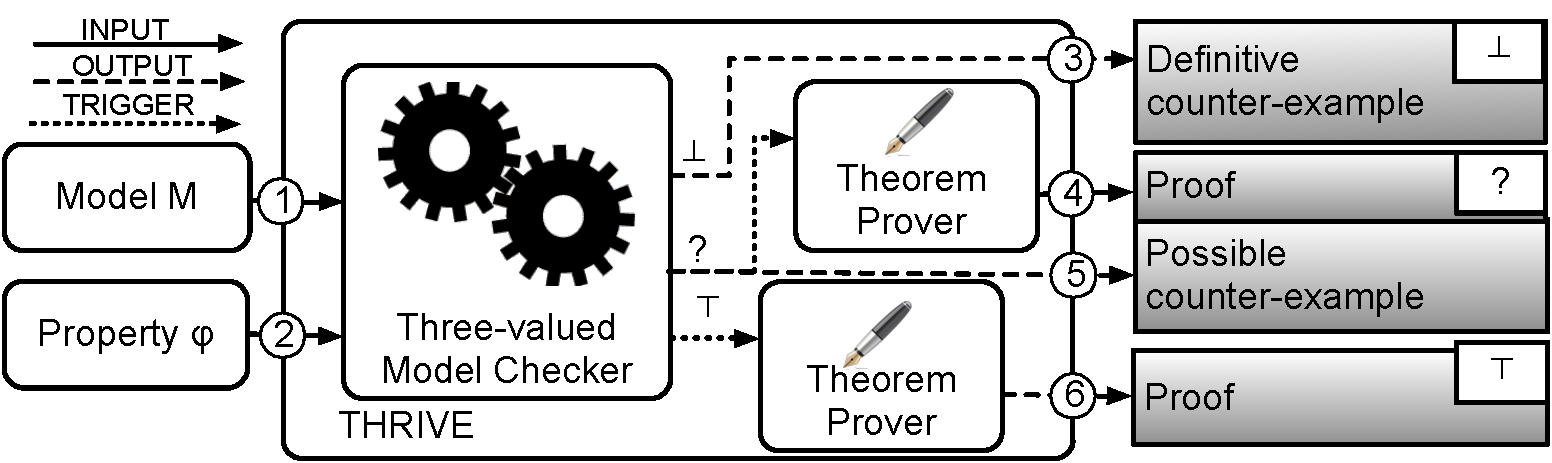
\includegraphics[width=\linewidth]{./images/atvaFig.pdf}
\end{center}
\caption{The \NAME\ framework.}  
\label{Fig.3vdv}
\end{figure}













\section{Using \NAME\ with PKS and LTL}
\label{sec:theoremProverAdapting}
This section describes the instance of \NAME\ proposed in this paper, using PKSs and and LTL. We first show how we modified the theorem prover framework presented in Section~\ref{sec:preliminaries} to support PKSs and how it is integrated with the three-valued model checker. We further analyze the case of thorough semantics, which is more appealing in practice, and discuss to what extent and how the framework can be used in such a case.
% and the theorem prover;
%\item the correctness of the integrated framework considering the three-valued and the thorough LTL semantics also for the subset of self-minimizing LTL formulae.
%\end{enumerate*}




\subsection{Adapting the theorem prover.}
\label{sec:adapting}
The deductive verification framework presented in~\cite{peled2001model}  exploits the product between a state labeled transition system and  a GBA \gba\ obtained by $\lnot\phi$ to generate the proof.
To enable the algorithm to work on KSs and BAs, 
we describe
%it is necessary to specify
 how to associate LTL formulae with each state of the BA and how to identify failed states of the product automaton.

\vskip 0.05in  
\textbf{Identification of the formulae that hold in the states of  the BA.}
We assume that the degeneralization procedure~\cite{clarke1999model}, that converts the GBA  \gba\
%$\mathcal{G}$ 
 into an equivalent BA \ba\
 %$\mathcal{A}$,
  behaves as follows: when a new state $q$ of 
  %$\mathcal{A}$
  \ba\ is created from a state $q^\prime$ of 
  \gba ,
  %$\mathcal{G}$, 
the formulae $\eta(q^\prime)$ and $\mu(q^\prime)$ are also associated to $q$.

\vskip 0.05in  
\textbf{Identification of failed states.} 
Following the procedure mentioned in Section~\ref{sec:preliminaries}, the product automaton 
%$M\otimes\mathcal{A}$
$M\otimes \ba$
 between the KS $M$ and the BA 
 %$\mathcal{A}$ 
\ba\ is modified to also generate \emph{failed states}.
Specifically, the product is computed using the rules~\ref{eq:classicalTransition} and~\ref{eq:failedTransition}.
%
\vspace{-1cm}
\begin{multicols}{2}
\begin{equation}
\label{eq:classicalTransition}
 \inferrule{s\rightarrow t \land q \xrightarrow{L(t)}p}{\langle s,q \rangle \rightarrow \langle t,p \rangle}  
\end{equation}\break
\begin{equation}
\label{eq:failedTransition}
 \inferrule{s\rightarrow t \land q \xrightarrow{\cancel{L(t)}}p}{\langle s,q \rangle \dashrightarrow \langle t,p \rangle}  
\end{equation}
\end{multicols}
%
Rule~\ref{eq:classicalTransition} is the classical rule used to compute the product automaton. 
It specifies that the state of the product $\langle s,q \rangle$  moves to $\langle t,p \rangle$ only if the transition $q \xrightarrow{L(t)}p$ that moves the BA from  $q$ to $p$ has the same label of the state $t$ of $M$.
Rule~\ref{eq:failedTransition} specifies how to compute failed states.
It states that the failed state $\langle t,p \rangle$ is generated in the product  when a transition  that moves the BA 
%$\mathcal{A}$
 \ba\ from $q$ to $p$ is labelled differently with respect to the state $t$ reached by the model $\mathcal{M}$ when the transition $s\rightarrow t$ is fired.
This is indicated using the notation $q \xrightarrow{\cancel{L(t)}}p$.
For this reason, the transition $\langle s,q \rangle \dashrightarrow \langle t,p \rangle$  from $\langle s,q \rangle $ to $\langle t,p \rangle$ is dashed.
Let us consider the product presented in Figure~\ref{fig:productOpt}  computed from the KS $M_{opt}$ obtained from the PKS in Figure~\ref{fig:model} and the BA of Figure~\ref{fig:property}.
The transition $\langle s_0, q_0 \rangle$ to  $\langle s_1, q_1 \rangle$ of the product presented in Figure~\ref{fig:productOpt} is dashed, since the proposition $\overline{g}$ is false in $s_1$, while the labeling of the transition from $q_0$ to $q_1$ requires $\overline{g}$ to be true for the transition to be performed.

The set 
%$\mathcal{F}(M\otimes\mathcal{A})$ 
 $\mathcal{F}(M\otimes \ba)$ of the \emph{failed states} contains the states $\langle t, p \rangle$ obtained by applying rule~\ref{eq:failedTransition}.
Note that, as stated in Section~\ref{sec:preliminaries}, each failed state $\langle s, q \rangle$ is such that $s \models \mu(q) $.
For example, the state $\langle s_1, q_1 \rangle$ of the product  presented in Figure~\ref{fig:productOpt} is a failed state.
Indeed, $s_1$ satisfies the property $\mu(q_1)= g \LTLor \LTLnext \LTLfinally g$ associated with the state $q_1$.



%%%%%%%%%%%%%%
\begin{theorem}
\label{th:deductivecorrecteness}
The deductive verification procedure is correct.
\end{theorem}

\begin{proof}
We show that the states identified as \emph{failed}  correspond to the ones that would be identified using~\cite{peled2001model}. 
In~\cite{peled2001model}, a state $\langle t, p \rangle$ is failed if the propositional assignment of $t$ does not satisfy the conditions specified in the state $p$. 
It is well known~\cite{gerth1996ltl2ba,clarke1999model}, that a GBA \gba\ associated with $\phi$ is such that
\begin{enumerate*}[label={(\arabic*)}]
\item all the transitions $(q,\alpha, p) \in \Delta$ that reach a state $p$ of the GBA have the same label $\alpha$ and that
\item a transition $(q,\alpha, p) \in \Delta$ is in the GBA  if and only if $\alpha$ satisfies the conjunction of the negated and non negated propositions that hold in the state $p$.
\end{enumerate*}
By construction, the latter of these properties also holds in the BA obtained from the GBA by applying the degeneralization procedure~\cite{clarke1999model}.
Thus, since all the transitions that reach $p$ are labelled with $\alpha$, a transition $\langle s,q \rangle \dashrightarrow' \langle t,p \rangle$ is added to the product automaton if and only if the propositional assignment of $t$ does not satisfy the propositional assignment specified in the state $p$. 
Furthermore, BAs acceptance condition is a special case of fairness condition used in~\cite{peled2001model}. 
Thus, the proposed deductive verification procedure is a special case of~\cite{peled2001model}, with regard to acceptance.\qed
\end{proof}

\begin{figure}[t]
\begin{minipage}[b]{.5\textwidth}
  \begin{figure}[H]
\centering




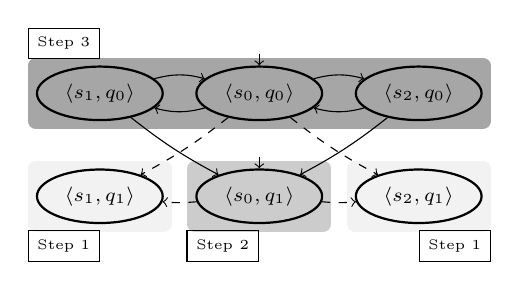
\begin{tikzpicture}[scale=0.33] %[x={10.0pt},y={10.0pt}]

\node[statep, initial, initial text={}, initial where=above] (s0q0) 
%[label={[yshift=-1.1cm,xshift=0cm]\scriptsize $\{q_0\}$},font=\scriptsize] {$\langle s_0,q_0\rangle$}; 
[font=\scriptsize] {$\langle s_0,q_0\rangle$}; 
\node[statep,  initial, initial text={}, initial where=above] (s0q1) 
%[below = 0.6cm of s0q0,label={[yshift=-1.1cm,xshift=0.5cm]\scriptsize $\{q_1\}$},font=\scriptsize] {$\langle s_0,q_1\rangle$}; 
[below = 0.6cm of s0q0,font=\scriptsize] {$\langle s_0,q_1\rangle$}; 

\node[statep] (s1q0) 
%[left = 0.4cm of s0q0,label={[yshift=-1.1cm,xshift=0cm]\scriptsize $\{q_0\}$},font=\scriptsize] {$\langle s_1,q_0\rangle$}; 
[left = 0.4cm of s0q0,font=\scriptsize] {$\langle s_1,q_0\rangle$}; 
\node[statep] (s1q1) 
%[below = 0.6cm of s1q0,label={[yshift=-1.1cm,xshift=0.5cm]\scriptsize $\{q_1\}$},font=\scriptsize] {$\langle s_1,q_1\rangle$}; 
[below = 0.6cm of s1q0,font=\scriptsize] {$\langle s_1,q_1\rangle$}; 

\node[statep] (s2q0) 
%[right = 0.4cm of s0q0,label={[yshift=-1.1cm,xshift=0cm]\scriptsize $\{q_0\}$},font=\scriptsize] {$\langle s_2,q_0\rangle$}; 
[right = 0.4cm of s0q0,font=\scriptsize] {$\langle s_2,q_0\rangle$}; 
\node[statep] (s2q1) 
%[below = 0.6cm of s2q0,label={[yshift=-1.1cm,xshift=-0.5cm]\scriptsize $\{q_1\}$},font=\scriptsize] {$\langle s_2,q_1\rangle$}; 
[below = 0.6cm of s2q0,font=\scriptsize] {$\langle s_2,q_1\rangle$}; 

%%LABELS for steps
\node[empty] (step3u) [above = 0.155cm of s0q0] {}; 
\node[empty] (step1u) [below = 0.155cm of s0q1] {}; 
\node[emptynode] (step3) [left = 1.9cm of step3u] {\tiny Step 3}; 
\node[emptynode] (step1) [left = 1.9cm of step1u] {\tiny Step 1}; 
\node[emptynode] (step1b) [right = 1.9cm of step1u] {\tiny Step 1}; 
\node[emptynode] (step2) [right= 1.1cm of step1] {\tiny Step 2};


\path[->]      
(s0q0) edge [bend left=15] node []{} (s1q0) 
(s1q0) edge [bend left=15] node []{} (s0q0)  

(s0q0) edge [bend left=15] node []{} (s2q0) 
(s2q0) edge [bend left=15] node []{} (s0q0)  

(s1q0) edge [bend right=5] node []{} (s0q1)
(s2q0) edge [bend left=5] node []{} (s0q1)

(s0q0) edge [bend left=5,dashed] node []{} (s1q1)
(s0q0) edge [bend right=5,dashed] node []{} (s2q1)

(s0q1) edge [bend left=5,dashed] node []{} (s1q1) 
(s0q1) edge [bend right=5,dashed] node []{} (s2q1) 
;    

\begin{pgfonlayer}{background}

%FAILED
\filldraw [line width=2mm,join=round,black!5]
(s1q1.south -| s1q1.west) rectangle (s1q1.north -| s1q1.east);
\filldraw [line width=2mm,join=round,black!5]
(s2q1.south -| s2q1.west) rectangle (s2q1.north -| s2q1.east);

%SUCCESSORS
\filldraw [line width=2mm,join=round,black!20]
(s0q1.south -| s0q1.west) rectangle (s0q1.north -| s0q1.east);

%INDUCTION
\filldraw [line width=2mm,join=round,black!35]
(s1q0.south -| s1q0.west) rectangle (s2q0.north -| s2q0.east);

\end{pgfonlayer}


\end{tikzpicture}

\caption{Product $I_{opt}=M_{opt}\otimes\mathcal{A}_{\lnot\phi_2}$}
\label{fig:productOpt}
 \end{figure}
\end{minipage}%
\begin{minipage}[b]{.5\textwidth}
  \begin{figure}[H]
\centering
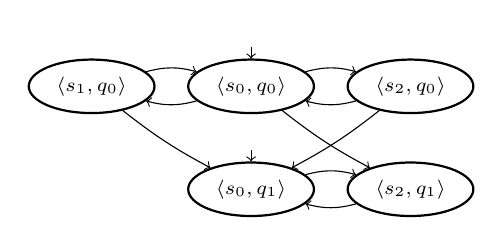
\begin{tikzpicture}[scale=0.33] %[x={10.0pt},y={10.0pt}]

\node[statep, initial, initial text={}, initial where=above] (s0q0) 
%[label={[yshift=-1.1cm,xshift=0cm]\scriptsize $\{q_0\}$},font=\scriptsize] {$\langle s_0,q_0\rangle$}; 
[font=\scriptsize] {$\langle s_0,q_0\rangle$}; 
\node[statep,  initial, initial text={}, initial where=above] (s0q1) 
%[below = 0.6cm of s0q0,label={[yshift=-1.1cm,xshift=0cm]\scriptsize $\{q_1\}$},font=\scriptsize] {$\langle s_0,q_1\rangle$}; 
[below = 0.6cm of s0q0,font=\scriptsize] {$\langle s_0,q_1\rangle$}; 

\node[statep] (s1q0) 
%[left = 0.4cm of s0q0,label={[yshift=-1.1cm,xshift=0cm]\scriptsize $\{q_0\}$},font=\scriptsize] {$\langle s_1,q_0\rangle$}; 
[left = 0.4cm of s0q0,font=\scriptsize] {$\langle s_1,q_0\rangle$}; 

\node[statep] (s2q0) 
%[right = 0.4cm of s0q0,label={[yshift=-1.1cm,xshift=0cm]\scriptsize $\{q_0\}$},font=\scriptsize] {$\langle s_2,q_0\rangle$}; 
[right = 0.4cm of s0q0,font=\scriptsize] {$\langle s_2,q_0\rangle$}; 
\node[statep] (s2q1) 
%[below = 0.6cm of s2q0,label={[yshift=-1.1cm,xshift=0cm]\scriptsize $\{q_1\}$},font=\scriptsize] {$\langle s_2,q_1\rangle$}; 
[below = 0.6cm of s2q0,font=\scriptsize] {$\langle s_2,q_1\rangle$}; 

\path[->]      
(s0q0) edge [bend left=15] node []{} (s1q0) 
(s1q0) edge [bend left=15] node []{} (s0q0)  

(s0q0) edge [bend left=15] node []{} (s2q0) 
(s2q0) edge [bend left=15] node []{} (s0q0)  

(s1q0) edge [bend right=5] node []{} (s0q1)
(s2q0) edge [bend left=5] node []{} (s0q1)

%(s0q0) edge [bend left=5,dashed] node []{} (s1q1)
(s0q0) edge [bend right=5] node []{} (s2q1)

%(s0q1) edge [bend left=5,dashed] node []{} (s1q1) 
(s0q1) edge [bend left=15] node []{} (s2q1) 
(s2q1) edge [bend left=15] node []{} (s0q1) 
;    

\end{tikzpicture} % pic 1
\caption{Product $I_{pes}=M_{pes}\otimes\mathcal{A}_{\lnot\phi_2}$}
\label{fig:productPess}
 \end{figure}
\end{minipage}%
\end{figure}
\subsection{Integrating the model checker and the theorem prover}
\label{sub:integrating}
Figure~\ref{Fig.3vdvinstance} presents an instance of \NAME\ obtained as an integration of a model checker for PKSs and LTL based on three-valued semantics and the theorem prover presented in Section~\ref{sec:adapting}. The circled numbers in Figure~\ref{Fig.3vdvinstance} indicate how this specific instance is plugged into \NAME\ in Figure~\ref{Fig.3vdv}.






The three-valued model checker presented in Section~\ref{sec:preliminaries} is used by \NAME\  to check the satisfaction of the property of interest.
Specifically, it runs twice a classical two-valued model checker, considering first the optimistic approximation $M_{opt}$, then the pessimistic approximation $M_{pes}$ of the PKS $M$.
When $M_{opt}$ is evaluated, if a counterexample is found, this is returned as output of \NAME .
Otherwise, \NAME\ verifies $M_{pes}$. 
If the property is satisfied, it means that no violating nor possibly violating behaviors have been identified.
Thus, \NAME\ executes the theorem prover that produces a proof that explains why no counterexample has been found in the pessimistic approximation.
Otherwise, the property is possibly satisfied.
In this case, \NAME\ returns the possible counterexample and runs the theorem prover on $M_{opt}$ to compute a proof that specifies why a definitive counterexample has not be found.




\begin{figure}[t]
\begin{center}         
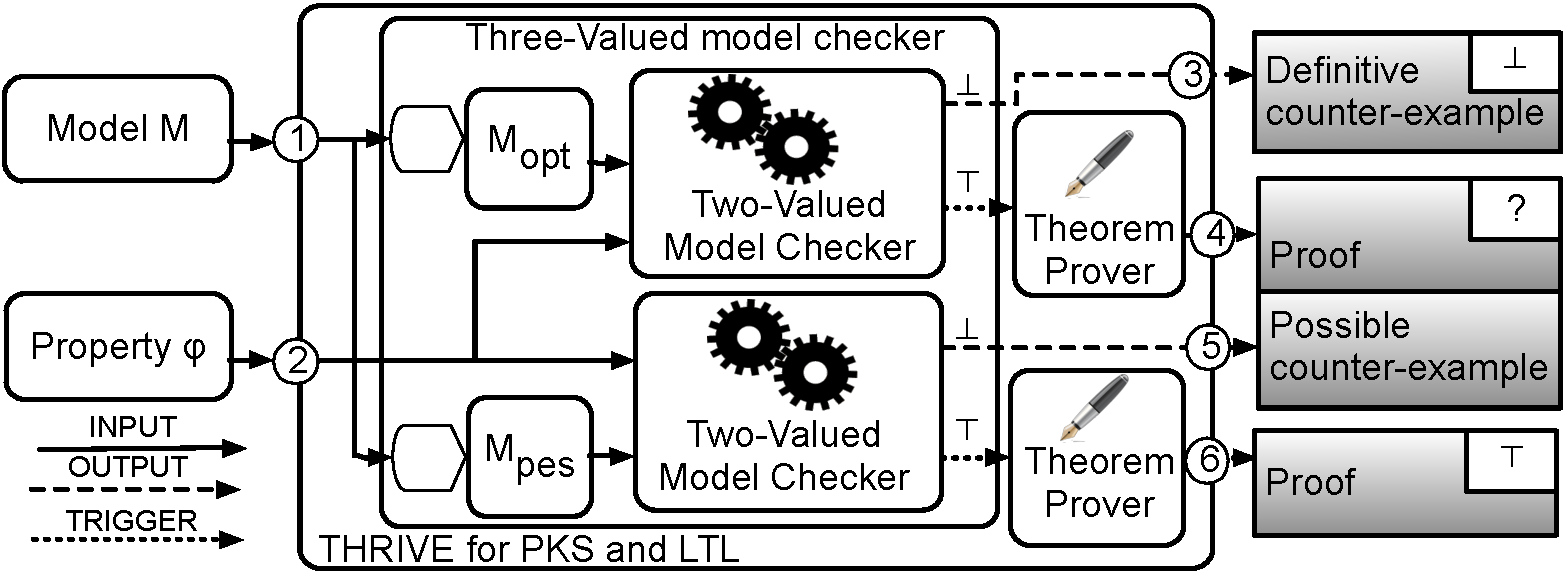
\includegraphics[width=\linewidth]{./images/atvaFigPKS.pdf}
\end{center}
\caption{\NAME\ for PKS and LTL.}  
\label{Fig.3vdvinstance}
\end{figure}



\textbf{Example}
%\emph{Consider properties $\phi_1$, $\phi_2$ and $\phi_3$ of the crossing semaphore example. They are satisfied, possibly satisfied and not satisfied, respectively, by the model $M$ of Figure~\ref{fig:model}.}
\emph{Properties $\phi_1$, $\phi_2$ and $\phi_3$ of the crossing semaphore example are satisfied, possibly satisfied and not satisfied by the model $M$ of Figure~\ref{fig:model}.}

\emph{
Property $\phi_2$.
The products between the optimistic and pessimistic approximation of the model $M$ and the BA automaton $\mathcal{A}_{\neg \phi_2}$ are presented in Figures~\ref{fig:productOpt} and~\ref{fig:productPess}.
\NAME\ explores $I_{pes}$ and returns the possible counterexample $(s_0, s_2)^\omega$.
Specifically,  by looping an infinite number of times on states $s_0$ and $s_2$ the green light is never turned on.
Since the property $\phi_2$ is possibly satisfied, the search of a definitive counterexample in the product automaton $I_{opt}$ (Figure~\ref{fig:productOpt}) fails.
%\NAME\ uses the product automaton $I_{opt}$ to compute a proof that explains the motivation.
%The obtained proof is presented in Table~\ref{table:proof}.
\NAME\ uses the product automaton $I_{opt}$ to compute a proof (Table~\ref{table:proof}) that explains the motivation.
The states that are analyzed in different steps are circled  in Figure~\ref{fig:productOpt} through different grey frames.
(\emph{Step1}). \NAME\ analyzes the failed states.
Given a failed state $\langle s, q \rangle$, since in this state the search for a counterexample fails, the formula associated with the state $q$ of $\mathcal{A}_{\lnot\phi_2}$ holds in $s$.
For example, since the state $\langle s_1, q_1 \rangle$ of $I_{opt}$ is a failed state, the formula $green \LTLor \LTLnext \LTLfinally green$ (valid in $q_1$) is satisfied by the model state $s_1$.
This formula is effectively true in $s_1$ since the green light is on.
(\emph{Step2}). Since all the successors of $\langle s_0, q_1 \rangle$ satisfy $green \LTLor \LTLnext \LTLfinally green$, it is possible to deduce that this property is also satisfied in $s_0$.
(\emph{Step3}). 
%The induction rule is applied considering the strongly connected component  $\left \{ \langle s_0, q_0 \rangle, \langle s_1, q_0 \rangle, \langle s_2, q_0 \rangle \right \}$.
%The rule allows to conclude that $s_0$ satisfies the property $\LTLnext \LTLglobally \LTLfinally green$.
The induction rule is applied considering the strongly connected component  $\left \{ \langle s_0, q_0 \rangle, \langle s_1, q_0 \rangle, \langle s_2, q_0 \rangle \right \}$ and  allows concluding that $s_0$ satisfies the property $\LTLnext \LTLglobally \LTLfinally green$.
(\emph{Step4}). \NAME\ applies the conjunction rule to $s_0$.
Since $s_0$ satisfies both $\LTLnext \LTLglobally \LTLfinally green$ and $green \LTLor \LTLnext \LTLfinally green$, it is possibly to deduce that $s_0$ satisfies the property $\phi_2$.
This provides an interesting insight to the designer: if she/he turns the green light on in $s_2$ the property becomes satisfied. The proof clearly states why.}

\emph{Property $\phi_3$. \NAME\ returns the counterexample $(s_0, s_1)^\omega$.
The counterexample specifies that by looping an infinite number of times on states $s_0$ and $s_1$ the green light is not permanently  on after the red. }

\emph{Property $\phi_1$. \NAME\  produces a proof that highlights how and why a definite counterexample is not found in the graph. First, it identifies the states $\langle s_0, q_1 \rangle$ and $\langle s_2, q_1 \rangle$ as failed. The conclusions found on these states are propagated to the state $\langle s_1, q_1 \rangle$. All the successors of the SCC formed by the product states related to the property state $q_0$ are analyzed. Finally, conclusions are drawn also on this SCC. 
The proof is omitted for space reasons.
}



\begin{table}[t]
\centering
\caption{Proof that $\phi_2$ is not violated.}
\label{table:proof}
\begin{tabular}[b]{ | P{2.5cm} | P{2.1cm} | P{3.3cm} | P{3cm} |  }
\hline
\emph{Step 1} &
\emph{Step 2} &
\emph{Step 3} &
\emph{Step 4}\\
\hline
%%\multicolumn{4}{|c|}{Steps}  \\
%% \hline
\textbf{Fail} & 
\textbf{Successors} &
\textbf{Induction} &
\textbf{Conjunction}\\
 \hline
\mbox{ $\langle s_2,q_1\rangle, \langle s_1,q_1\rangle$}
 &
 $\langle s_0,q_1\rangle$ 
 &
 $\mathcal{X}=\{\langle s_0,q_0\rangle,$ $ \langle s_1,q_0\rangle,\langle s_2,q_0\rangle\}$\newline
 $Exit(\mathcal{X})=\{\langle s_0,q_1\rangle, $ $ \langle s_1,q_1\rangle,\langle s_2,q_1\rangle\}$
 &
The initial state $s_0$ \\	
 \hline
  \inferrule{\langle s_1,q_1 \rangle  \in \mathcal{F}(I_{opt})\\
 \langle s_2,q_1 \rangle \in \mathcal{F}(I_{opt})
}
{ s_1, s_2\models g \LTLor \LTLnext \LTLfinally g }
  & 
 \inferrule{s_0\rightarrow\{s_1,s_2\} \\
 s_1\models g \LTLor \LTLnext \LTLfinally g \\
 s_2\models g \LTLor \LTLnext \LTLfinally g }
 {s_0\models g \LTLor \LTLnext \LTLfinally g} 
  &
\mbox{   \inferrule{ 
 s_0,s_1,s_2\models g \LTLor \LTLnext \LTLfinally g \\
s_0\rightarrow \{s_1,s_2 \} \\\\
 s_1\rightarrow \{s_0 \} \\\\
 s_2\rightarrow \{s_0 \}   
   }
{s_0,s_1,s_2\models \LTLnext \LTLglobally \LTLfinally g }}
  &
\inferrule{
 s_0\models \LTLnext \LTLglobally \LTLfinally g \\
  s_0\models g \LTLor \LTLnext \LTLfinally g \\
 \LTLnext \LTLglobally \LTLfinally g \LTLand  (g \LTLor  \LTLnext \LTLfinally g)\rightarrow \phi_2 }
 {s_0\models \phi_2}
\\  
\hline

\end{tabular}
\end{table}

\subsection{Thorough semantics and \NAME}
As stated in Section~\ref{sec:preliminaries},  three-valued semantics does not always behave in accordance with the natural intuition~\cite{bruns2000model}.
When $\phi$ possibly holds in $M$,   it is desirable that there exist two completions $M^\prime$ and $M^{\prime\prime}$ of $M$  such that $M^\prime$ satisfies  $\phi$  and   $M^{\prime\prime}$ violates $\phi$.
This property is not ensured by the three-valued semantics, and is the motivation that leads to introduce thorough LTL semantics. Hereafter, we discuss how the adoption of thorough semantics would affect the use of the \NAME\ framework.

Given a PKS  $M$ and a property  $\phi$,  \NAME\ produces the following outputs:

\noindent \emph{Property is satisfied.}
%In this case, \NAME\ works correctly. 
\NAME\ works correctly. 
A property $\phi$ that evaluates to $\LTLtrue$ under three-valued semantics is also satisfied under thorough semantics.
Thus, the  verification result is correct.
Also the proof is correct since it shows that any completion of $M$ satisfies $\phi$. 

\noindent \emph{Property is not satisfied.}
%In this case, \NAME\ works correctly. 
 \NAME\ works correctly. 
When the model checker returns a $\LTLfalse$ value, the counterexample shows a behavior that violates $\phi$.
A property $\phi$  that is not satisfied considering the three-valued semantics, is also not satisfied considering the thorough semantics.
%Thus, the counterexample is a correct counterexample that proves the existence of a completion of $M$ that violates $\phi$.
Thus, the counterexample is correct and proves the existence of a completion of $M$ that violates $\phi$.
 
\noindent \emph{Property is possibly satisfied.}
%This case is not handled by \NAME\ correctly for all LTL properties.
 \NAME\ does not work correctly  for all LTL properties. 
When the three-valued model checker returns  $?$  the property is possibly satisfied considering the three-valued semantics but no conclusion can be drawn based on thorough semantics.
Indeed, there are cases in which a $?$ is returned, but all the completions of the model either satisfy or do not satisfy $\phi$. 
The computed counterexample and proof can be spurious under the thorough semantics.


%In this case, if a correct result is required, the use of a generalized model checking procedure~\cite{bruns2000model} (not discussed here) becomes necessary. 
%Since when a property $\phi$ is evaluated to $?$ there could exist a completion that violates $\phi$, the produced proof is not correct.

%
%
%Correctness is analyzed by comparing the results returned by \NAME\ with the  results  that would be returned considering the thorough LTL semantics.
%We stated that a model checking result---the verification result, the counterexample or the possible counterexample---is \emph{correct} (\validCounterexample ) if it corresponds to the results that would be obtained considering the thorough LTL semantic.
%Otherwise, it is \emph{incorrect} (\spuriosCounterexample), i.e., the counterexample can be spurious.
%We stated that a proof generated by \NAME\ is \emph{correct} (\validProof) if it proves the satisfaction/possibly satisfaction of a property considering the thorough LTL semantics. 
%Otherwise, it is \emph{incorrect} (\notvalidProof ).
%Table~\ref{tab:results} shows the comparison. 
%The rows of the table specify whether \NAME\ states that the property of interest is satisfied ($\LTLtrue$), possibly satisfied ($?$) or not satisfied ($\LTLfalse$).
%If the property is satisfied/possibly satisfied Table~\ref{tab:results} considers the correctness of the verification result ($\LTLtrue$, $?$ or $\LTLfalse$) and the proof.
%If the property is not satisfied only the correctness of the verification result is considered since no proof is produced.
%The correctness of the framework w.r.t. LTL properties is presented by the column with labeled as LTL.

%\textbf{Property satisfied.}
%When a property $\phi$ is evaluated to $\LTLtrue$ considering the three-valued semantics, it is also satisfied considering the thorough semantics.
%Thus, the  verification result is correct.
%Also the proof is correct since it shows that any completion of $M$ satisfies $\phi$. 
%
%\textbf{Property not satisfied.}
%When the model checker returns a $\LTLfalse$ value, the counterexample shows a behavior that violates $\phi$.
%A property $\phi$  that is not satisfied considering the three-valued semantics, is also not satisfied considering the thorough semantics.
%Thus, the counterexample is a correct counterexample that proves the existence of a completion of $M$ that violates $\phi$.
% 
%\textbf{Property possibly satisfied.}
%When the three-valued model checker returns a $?$ value the property is possibly satisfied considering the three-valued semantics but no conclusion can be achieved by considering the thorough semantics.
%Indeed, there are cases in which a $?$ is returned but all the completions of the model either satisfy or do not satisfy the property of interest. 
%The computed counterexample can be a spurious counterexample under the thorough semantics.
%The corresponding cell in Table~\ref{tab:results} is marked with a \spuriosCounterexample\ symbol meaning that the counterexample is not correct.
%In this case, if a correct result is required, the use of a generalized model checking procedure~\cite{bruns2000model} (not discussed here) becomes necessary. 
%Since when a property $\phi$ is evaluated to $?$ there could exist a completion that violates $\phi$, the produced proof is not correct.


%
%\begin{table}[t]
%\centering
%\caption{LTL and self-minimizing LTL validity of the framework outputs.}
%\label{tab:results}
%\begin{tabular}{   c  c | c | c | }
%\cline{1-4}
%  \multicolumn{1}{| c }{Result} & \multicolumn{1}{| c |}{Type of Output} & \multicolumn{1}{c |}{LTL} & \multicolumn{1}{c |}{Self-minimizing LTL} \\
%\cline{1-4} 
%  \multicolumn{1}{| c }{\multirow{2}{*}{$\LTLtrue$}} &  \multicolumn{1}{| c |}{Verification result} & \multicolumn{1}{ c |}{\validCounterexample}  & \validCounterexample  \\
%    \cline{2-4}
% \multicolumn{1}{| c }{} &  \multicolumn{1}{| c |}{Proof} & \validProof  & \validProof  \\
%  \cline{1-4}
%  \multicolumn{1}{| c }{\multirow{2}{*}{$?$}} &  \multicolumn{1}{| c |}{Verification result}  & \multicolumn{1}{ c |}{\spuriosCounterexample} & \validCounterexample  \\
%  \cline{2-4}
%  \multicolumn{1}{| c }{} &  \multicolumn{1}{| c |}{Proof} & \notvalidProof\  & \validProof  \\
%   \cline{1-4}
% \multicolumn{1}{| c }{$\LTLfalse$} & \multicolumn{1}{| c |}{Verification result} &  \multicolumn{1}{ c |}{\validCounterexample} & \validCounterexample   \\
% \hline
%\end{tabular}
%\end{table}
% 
%
\textbf{Example.}
\emph{The results obtained for $\phi_1$ and $\phi_3$ of the crossing semaphore example are correct both considering the three-valued and the thorough semantics. 
Since $\phi_1$ is satisfied, the proof is a correct proof that justifies why all the completions of the model presented in Figure~\ref{fig:modelmot} satisfy $\phi_1$.
The counterexample  returned for $\phi_3$ is correct, i.e., all the completions of the model presented in Figure~\ref{fig:modelmot} exhibit the behavior returned as a counterexample.}


\vskip 0.05in  
\textbf{Self-minimizing LTL formulae.} 
Self-minimizing LTL formulae are a subset of LTL formulae that present an interesting property:  three-valued and  thorough semantics are equivalent, i.e., if $\phi$ is self-minimizing, then $[(M, s) \models \phi]=[(M, s) \models \phi]_t$.
Therefore, the three-valued model checking framework presented in Section~\ref{sec:preliminaries} produces a result that is correct also considering the thorough semantics. 
For this reason, whenever the three-valued model checker returns $?$,  the proof and the possible counterexample produced by \NAME\ are also correct  under the thorough semantics. In~\cite{godefroid2005MCvsGMC}, the authors propose a first grammar for this LTL subset. 
The grammar does not capture entirely this set. However, it can be used to generate formulae that are self-minimizing by construction, or to check whether a formula is self-minimizing (sufficient condition). 
Furthermore, the authors argue that the set of self-minimizing LTL formulae contains most property patterns of practical interest, such as absence, universality, existence, response and response chain~\cite{dwyer1998property}. 
%For these reasons it is  possible in practice to use the version of \NAME\ of Figure~\ref{Fig.3vdvinstance} also under the thorough semantics interpretation.
For these reasons it is  possible in practice to use the version of \NAME\ of Figure~\ref{Fig.3vdvinstance} also considering the thorough semantics.


\textbf{Example}
\emph{Property $\phi_2$ is a special instance of LTL response pattern which, according to~\cite{godefroid2005MCvsGMC}, is self-minimizing.
Thus, the possible counterexample and the proof returned by \NAME\ are correct.}









%\label{sec:example}
%



















\section{Preliminary evaluation}
\label{sec:preliminaryEvaluation}
This section tries to answer the following research question: \emph{how effective is \NAME\ w.r.t. incremental development?}

To provide an initial answer, we simulated the design of a critical software system. 
The system, described in~\cite{arcaini2015formal}, is used by optometrists and ophtalmologists to test visual problems and certify a certain level of stereoacuity.
The test requires patients to pass levels with increasing difficulties, in which they have to recognize images.
Each time the patient is able to recognize an image the system shifts to a higher level and a more difficult image is shown. 
When the patient fails, the level is decreased.
The test ends in one of these cases:
\begin{enumerate*}
\item when the patient fails the image recognition and she/he did not pass an easier level;
\item when the top level is reached;
\item if the doctor interrupts the test.
\end{enumerate*}
The complete model and the obtained results can be found in~\cite{bernasconi2017example}.
 

\textbf{Experimental setup.}
We modelled the system in~\cite{arcaini2015formal} as a PKS. 
For simplicity we considered only two levels. 
We used the atomic propositions \textit{fl}, \textit{sl}, \textit{test}, \textit{edb}, \textit{cert} and \textit{uncert} to specify that 
the patient is in the first or in the second level of the test, 
the test is under execution,
a mistake has been made by the patient, 
the patient has been certified and the patient is not certified, 
respectively.
If at some point the doctor quits the test, the patient is not certified.
If the patient fails the first level, the patient is not certified.
If he/she passes the first level, the second level is entered. 
If the patient also passes the second level he/she is certified at the second level.
Otherwise, we assume that the designer is uncertain on the level in which the component should certify/not-certify the patient (this is formalized by setting $fl=?$, $sl=?$).

We designed a set of properties that the system has to satisfy.
\begin{enumerate*}
\item[] Property $\psi_1=(\neg cert) \LTLweakuntil$ $(\neg sl)$ states that a patient is not at the second level before he/she is certified (see~\cite{ltlpatternsurl}). Note that, as observed in the following, this property is wrong.
\item[] Property  $\psi_2=\LTLglobally(test \rightarrow \LTLfinally(cert \LTLor uncert))$ specifies that every test must be followed by a certification or a non-certification.
\item[] Property  $\psi_3=\LTLglobally(edb \rightarrow \LTLfinally (cert \LTLor fl))$ states that if an error has been made by the patient (\emph{edb}), she/he cannot be uncertified and be at the second level ($\neg fl$). Indeed, a mistake prevents a patient from increasing the assessed level.
\end{enumerate*}
Note that these properties are obtained from well-known property patterns~\cite{dwyer1998property}.


\textbf{Results.} \emph{Property $\psi_1$.} 
 \NAME\  returns the value $\LTLfalse$ and returns a definitive counterexample showing that there exists a case in which a patient is assessed at the second level but has not been certified yet.
Indeed, the property is wrong; the desired property should have been expressed  as $\neg(cert \LTLand fl) \LTLweakuntil (\neg sl)$, meaning that a patient is not at the second level before he/she is certified at the first level.

\emph{Property $\psi_2$.}  \NAME\ returns the value $\LTLtrue$, since the property of interest is satisfied. 
The proof shows that a $test$ is always followed by a $cert$ or $uncert$.


\emph{Property $\psi_3$.} 
\NAME\ returns the value $?$ and a possible counterexample obtained by assigning $\LTLfalse$ to the proposition \emph{fl}. 
\NAME\ considers the optimistic approximation to produce a proof that no definitive counterexample can be found.
The obtained proof is correct since a simple grammar check shows that $\psi_3$ is self-minimizing. The proof shows why, by assigning $\LTLtrue$ to the unknown proposition \emph{fl}, the property of interest is satisfied.
%First, it identifies the failed states, in which the property $\lnot cert \LTLand \lnot sl \LTLor edb$ holds. 
%Then, the successors and the induction rules are iteratively applied.
%Finally, conclusions are deduced for the initial state of the model. 

The feedback produced by \NAME\ for properties $\psi_1$, $\psi_2$ and $\psi_3$ successfully helps in understanding whether a property of interest is satisfied, possibly satisfied or violated. 
When the property is satisfied/possibly satisfied, understanding the reason why this is true supports self-confidence.

%\fixme{I don't like the "threats to validity". I would drop it or simply say that we have used one small example here, and more should be done, especially with 2real" cases of software development. Perhaps we can refer to other works that try to manage in a similar way un+certainty in sw development.}

%\textbf{Threats to validity.}  The proposed model is obtained by changing the values of some propositions to a $?$ value. 
%There is no guarantee that the designer was  uncertain about the values of these propositions during the development. 
%However, the proposed changes have been applied trying to simulate reasonable doubts the designed can have during the development.






\section{Using \NAME\ in real cases}
\label{sec:discussion}
%\fixme{I suggest that we get rid of this section. Almost all comments on self-minimizing have already been moved to earlier. I do not understand the comment on the available grammar for self-minim LTL formulae. If there is a grammar that precisely defines them, why not use it instead of the LTL grammar? But then below you also say that checking whether an LTL formula is self-min is expensive--exponential. How can it be if we have a simple grammar? There is something fishy here. I suggest that you extract the few useful comments that are still worth making and perhaps move to conclusions (with future work). For example, the fact that we could build a model checker for thorough semantics might go there. The final comment on scalability may perhaps instead go earlier to 4.3}


This section elaborates on the applicability of \NAME\ in real cases. 

\emph{Three-valued vs thorough semantics.} %When  \NAME\ returns a $?$ value, the result is not correct considering the thorough semantics.
The generalized model checking algorithm~\cite{bruns2000model} (which levies a performance penalty) could be used to check a property under the thorough semantics.
In~\cite{gurfinkel2005thorough}, the authors analyze how the generalized model checking really helps.
Whenever the model is built using predicate abstraction~\cite{graf1997construction}, the thorough check does not provide additional precision.
It is also argued that in many practically interesting cases, the thorough semantics is not more precise than the three-valued one. 
For these reasons, \NAME\ can be correctly applied in most of the real world cases.

\emph{Temporal patterns of self-minimization.} 
%\NAME\ always produces a correct result when the LTL formula is self-minimizing.
%In~\cite{godefroid2005MCvsGMC} the authors propose a first grammar for this LTL subset.
%This grammar can be used to generate formulae that are (by construction) self-minimizing or to check whether a specific formula is self-minimizing.
%The authors also argue that the set of self-minimizing LTL formulae contains most of the properties of practical interest, such as absence, universality, existence, response and response chain. 
In~\cite{antonik2006efficient}, the authors consider popular syntactic specification patterns, documented at a community-led pattern repository, and check whether formulae compliant with these patterns are self-minimizing.
They show that many such patterns are self-minimizing and the ones that are not can be transformed with linear blowup into a self-minimizing LTL formula.
Thus, in most practical cases, the designer will consider a formula that is self-minimizing. 
A syntactic check can be used to prove self-minimization before running \NAME .

\emph{Checking whether an LTL formula is self-minimizing.} Checking whether an LTL formula is self-minimizing is expensive, since it requires to compute an automaton that is exponential in $|\phi|$~\cite{godefroid2005MCvsGMC}. 
However, if $\phi$ satisfies some constraints (sufficient conditions) then it is self-minimizing.
For example, if it is in its negation normal form and no proposition occurs in mixed polarity, then $\phi$ is self-minimizing.
These checks can be implemented in \NAME . 

\emph{Scalability.} Three-valued model checking is as expensive as classical model checking~\cite{bruns1999model}, which is commonly used to analyze real world problems~\cite{Woodcock:2009:FMP:1592434.1592436}.
Deductive verification has been employed successfully in the verification of digital hardware and software systems~\cite{rajan1995integration}.
%However, there are inherent limits to the efficiency with which expressive general-purpose logics can be fully mechanized. 
%Two approaches have been proposed in literature to overcome this limitation:
%\begin{enumerate*}
%\item  using interactive deductive verification tools so that correctness proofs can be developed through a combination of user guidance and limited forms of automated deduction;
%\item considering useful fragments of logic that can be mechanized very effectively.
%\end{enumerate*}
Since \NAME\ simply combines multi-valued model checking and theorem proving, its scalability improves  as the performance of the employed model checking and deductive verification  frameworks enhances.




%\section{Related Work}
%\label{sec:stateoftheart}
%





\section{Conclusions and future work}
\label{sec:conclusions}
This work presented \NAME, a theoretical framework for a correct integration of existing multi-valued model checkers and theorem provers. 
Whenever the property of interest is definitely satisfied, or possibly satisfied, \NAME\ provides  information regarding why a certain result is returned by the model checker.
The proof gives intuition on what is working correctly in the current design and insights for the next development rounds.
We instantiate \NAME\ considering a PKS, to express the model of the system, and LTL, to specify the property of interest. 
We show that the instantiation is feasible and sound, and requires changing the model checking algorithm to accomodate the execution of the theorem prover.
\NAME\ has been evaluated considering a safety critical example~\cite{arcaini2015formal}, which showed  the effectiveness  of the approach. 
We also discussed the applicability of the approach in real world cases.

As future work, we aim to implement \NAME\ by integrating existing model checkers and theorem provers. 
This  will allow us to provide further evidence of the impact of \NAME\ in continuous system development and to analyze the challenges of realistic systems.
We would like to introduce possible extensions of the currently considered formalisms: other forms of partial systems models and other multi-valued logic options for the properties.
Finally, we also wish to investigate thoroughly how the proofs can be written in the most understandable and useful form for the designer.




\subsubsection*{Acknowledgments.} 
Research partly supported from the EU H2020 Research and
Innovation Programme under GA No. 731869 (Co4Robots).

\bibliographystyle{abbrv}
\bibliography{sigproc} 

\end{document}
 





